
%----------------------------------------
\begin{frame}[fragile]
  \frametitle{Second application}

{\Large\bf Using Temporal Constraints to Generate Schedules}

\end{frame}

%----------------------------------------
\begin{frame}[fragile]
  \frametitle{Inspiration: the MEXEC scheduling system}

\begin{figure}
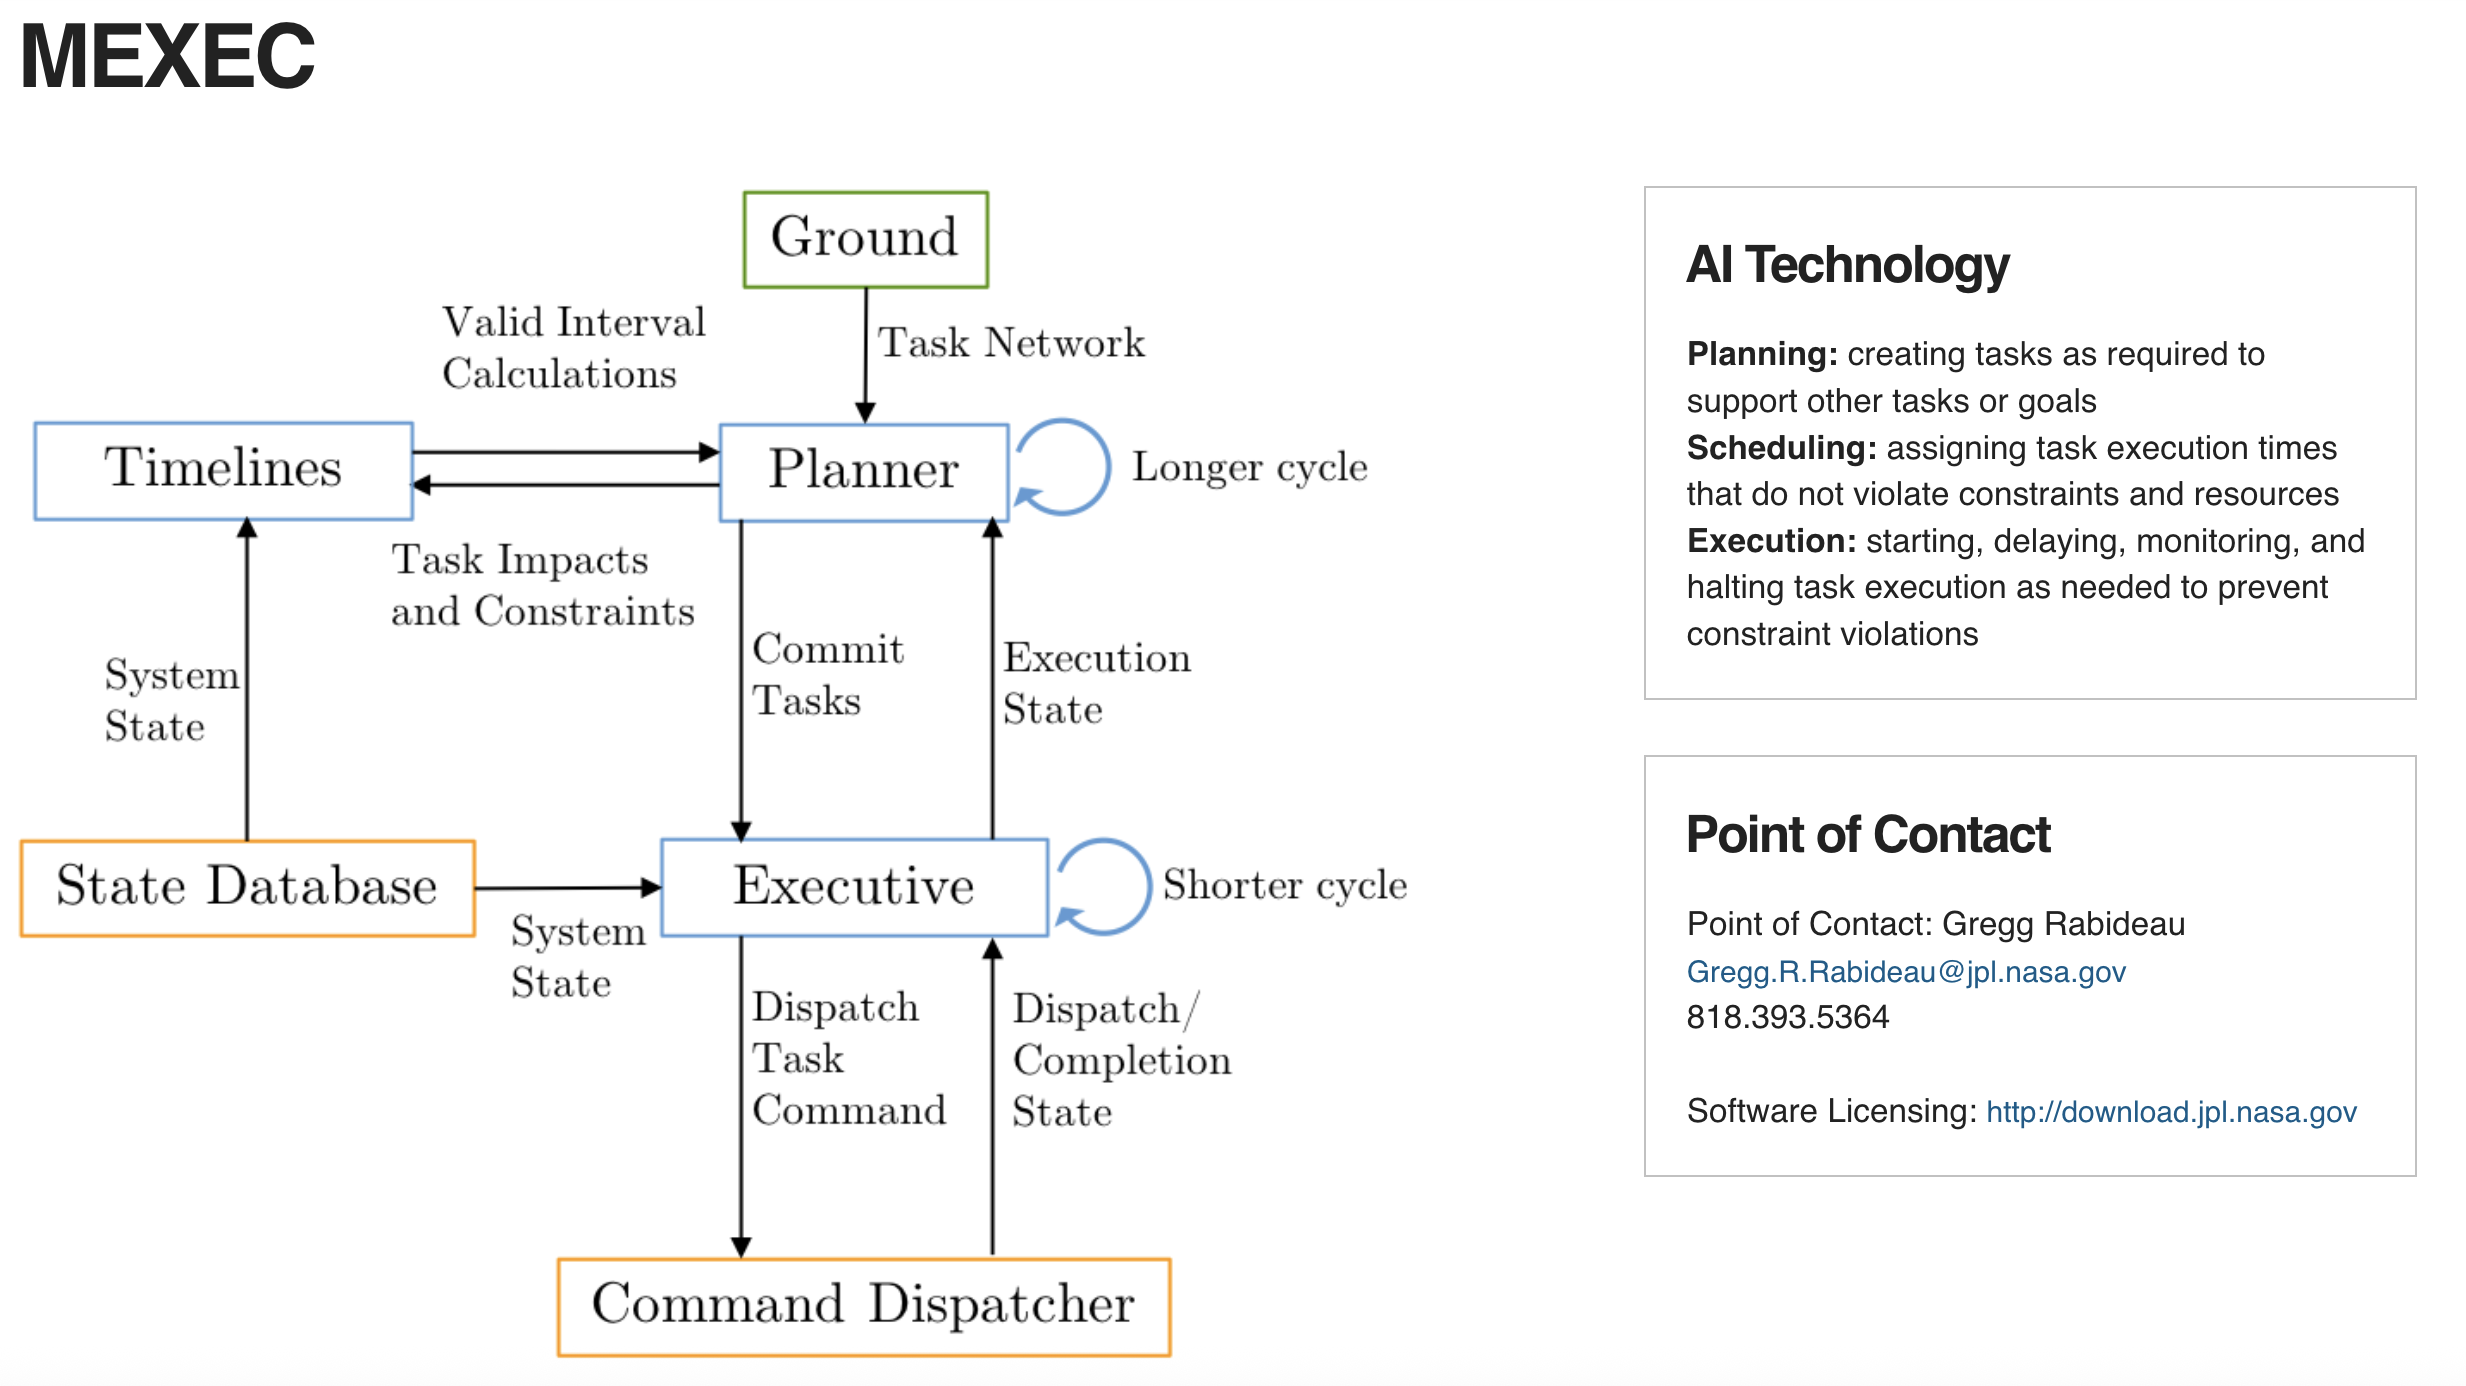
\includegraphics[width=1.0\textwidth]{figures/mexec.png}
%\caption{Your caption}
\end{figure}

\end{frame}

%----------------------------------------
\begin{frame}[fragile]
  \frametitle{A tasknet: timelines} \small

\begin{lstlisting}[language=tasknetdsl,frame=single]
tasknet Rover {
  end = 400;

  timelines {
    arm : atomic = false;
    location : state(home, target) = home;
    data : cumulative [0.0, 50.0] bounds [0.0, 100.0] = 0.0;
    battery : rate [10.0, 100.0] bounds [0.0, 100.0] = 60.0;
    temperature : rate [5.0, 40.0] bounds [0.0, 100.0] = 10.0;
  }

  task drive { ... }
  task collect { ... }
  optional task charge { ... }
  optional task heating { ... }
}
\end{lstlisting}

\end{frame}

%----------------------------------------
\begin{frame}[fragile]
  \frametitle{A tasknet: tasks} \small

\begin{lstlisting}[language=tasknetdsl,frame=single]
  task drive {
    startrange [100, 120];
    endrange [130, 160];
    durationrange [30,40];

    pre {
      battery in [60.0, 100.0]; 
      temperature in [10.0, 40.0]; 
    }

    impacts {
      maint {
        battery +~ -1.5;  
      }
      post {
        location = target;
      }
    }
  }
\end{lstlisting}

\end{frame}

%----------------------------------------
\begin{frame}[fragile]
  \frametitle{A tasknet: tasks} \small

\begin{lstlisting}[language=tasknetdsl,frame=single]
  task collect {
    durationrange  [20, 30];

    pre {
      location = target;
      battery in [60.0, 100.0];
      arm = false;
    }

    impacts {
      pre {
        arm = true;
      }
      maint {
        battery +~ -0.5; 
        temperature +~ -0.2;
      }
      post {
        data += 40.0; 
        arm = false;
      }
    }
  }
\end{lstlisting}

\end{frame}

%----------------------------------------
\begin{frame}[fragile]
  \frametitle{A tasknet: optional tasks} \small

\begin{lstlisting}[language=tasknetdsl,frame=single]
 optional task charge {
    durationrange [60,70];

    pre {
      battery in [0.0, 60.0];
    }

    impacts {
      maint {
        battery +~ 2.0; 
      }
    }
  }

  optional task heating {
    duration_range [10, 10];

    impacts {
      maint {
        battery +~ -0.5; 
        temperature +~ 2; 
      }
    }
  }  
\end{lstlisting}

\end{frame}

%----------------------------------------
\begin{frame}[fragile]
  \frametitle{A tasknet: temporal constraints and properties} \small

\begin{lstlisting}[language=tasknetdsl,frame=single]
  constraints {
    prop charge_drive:   always not (active(charge) and active(drive));
    prop temperature10:  always temperature >= 10;
  }
\end{lstlisting}

\pause

\begin{lstlisting}[language=tasknetdsl,frame=single]
  properties {
    prop target_reached: eventually (location = target and data >= 30);
    prop drive_charge:   always (active(drive) -> eventually active(charge));
    prop temperature:    always temperature >= 10;
  }
\end{lstlisting}

\end{frame}

%----------------------------------------
\begin{frame}[fragile]
  \frametitle{A generated schedule} \small

\begin{verbatim}
Schedule for TaskNet `Rover3`:
  drive         : start =  118, end =  148
  heating       : start =  137, end =  147
  charge        : start =  149, end =  209
  collect       : start =  210, end =  233

PROPERTY 'target_reached' HOLDS
PROPERTY 'drive_charge' HOLDS
PROPERTY 'temperature' HOLDS
\end{verbatim}

\end{frame}

%----------------------------------------
\begin{frame}[fragile]
  \frametitle{A Generated Schedule} \small

\begin{verbatim}
-- zone 1: (118, 137] --
    active tasks : drive
    arm            = False
    location       = home
    data           = 0
    battery        = 60 -> 31.5
    temperature    = 10 -> 10

  -- zone 2: (137, 147] --
    active tasks : drive, heating
    arm            = False
    location       = home
    data           = 0
    battery        = 31.5 -> 11.5
    temperature    = 10 -> 30
  ...
\end{verbatim}

\end{frame}

%----------------------------------------
\begin{frame}[fragile]
  \frametitle{The scheduling and the verification problem} \small

\begin{block}{The scheduling problem}
\[
\exists initial . \exists schedule . constraints(initial, schedule)
\]
\end{block}

\pause

\begin{block}{The verification problem, proving property $\varphi$ for all schedules}
\[
\forall initial . \forall schedule . constraints(initial, schedule) \rightarrow \varphi(schedule)
\]
\end{block}

\end{frame}

%----------------------------------------
\begin{frame}
  \frametitle{TaskSAT VS extension for syntax highlighting} \small

\begin{figure}
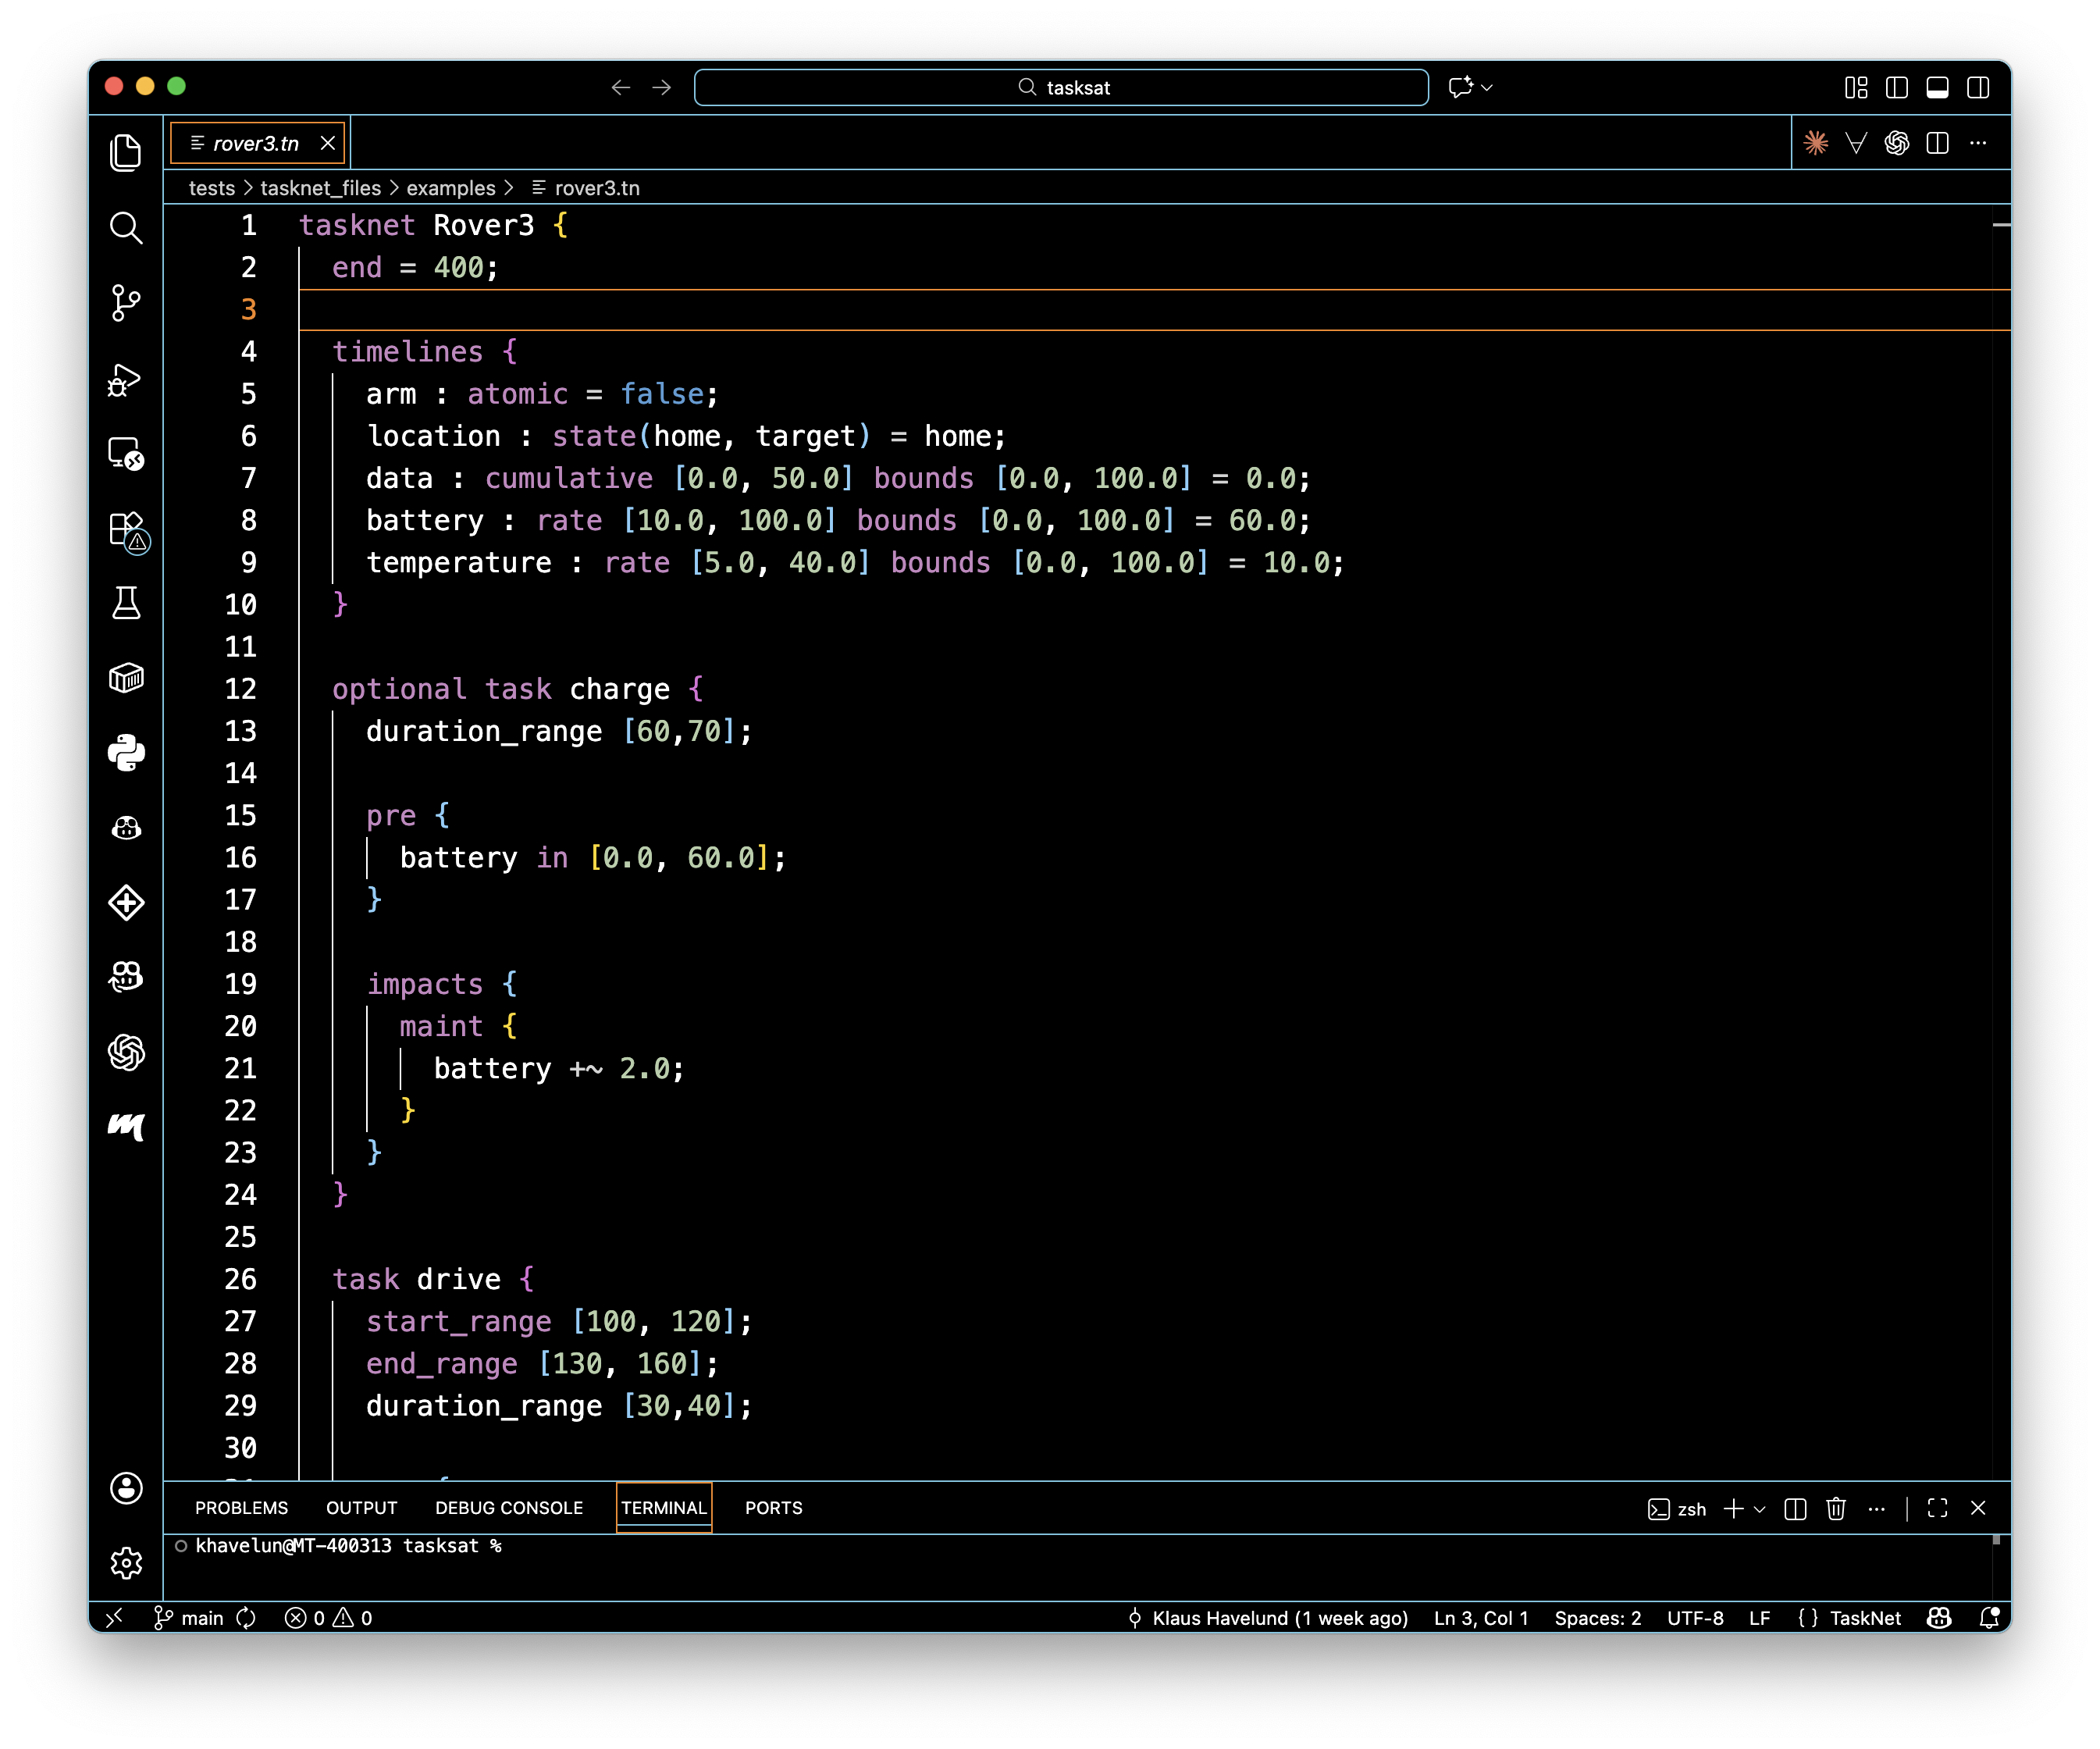
\includegraphics[width=0.85\textwidth]{figures/vs-code.png}
%\caption{Your caption}
\end{figure}

\end{frame}